\documentclass[aspectratio=169,10pt]{beamer}

\usetheme{Madrid}
\usecolortheme{seahorse}
\usefonttheme{professionalfonts}

\usepackage{amsmath,amssymb,amsthm}
\usepackage{mathtools}
\usepackage{listings}
\usepackage{xcolor}
\usepackage{booktabs}
\usepackage{graphicx}
\usepackage{algorithm}
\usepackage{algpseudocode}
\usepackage{array}

\graphicspath{{figures/}}

%% Python listing style
\lstdefinestyle{python}{
  language=Python,
  basicstyle=\ttfamily\scriptsize,
  keywordstyle=\color{blue!80!black}\bfseries,
  stringstyle=\color{orange!80!black},
  commentstyle=\color{green!50!black}\itshape,
  numberstyle=\tiny\color{gray},
  numbers=left, stepnumber=1,
  frame=single, breaklines=true,
  showstringspaces=false, tabsize=4,
  backgroundcolor=\color{gray!7},
}

\newcommand{\bbP}{\mathbb{P}}
\newcommand{\bbE}{\mathbb{E}}
\newcommand{\bbR}{\mathbb{R}}
\newcommand{\bbN}{\mathbb{N}}
\newcommand{\bbB}{\mathbb{B}}

\title[UAI -- Ch.2.5 Info.\ Theory]{An Introduction to Universal Artificial Intelligence}
\subtitle{Chapter 2: Background --- Section 2.5: Information Theory and Coding}
\author{Based on Hutter, Quarel \& Catt (2024)}
\date{}

\setbeamertemplate{navigation symbols}{}
\setbeamertemplate{footline}[frame number]

\begin{document}

% ------------------------------------------------------------------ title
\begin{frame}
  \titlepage
\end{frame}

% ------------------------------------------------------------------ TOC
\begin{frame}{Section 2.5 Outline: Information Theory and Coding}
  \tableofcontents[hideallsubsections]
\end{frame}

\section{2.5 Motivation}
\section{2.5.1 Shannon Entropy}
\section{2.5.2 Shannon-Fano Code}
\section{2.5.3 Kullback--Leibler Divergence}
\section{2.5.4 The Kraft Inequality}

%% ==================================================================
\begin{frame}[allowframebreaks]{2.5 Why Information Theory?}

We make observations all the time about the world around us, both through
direct first-hand observations and indirect inferences based on collected
data. Not all observations are equally ``informative''. If we already know
the outcome before it occurs, the information conveyed is useless.
Conversely, if the outcome is extremely surprising (unlikely), then learning
that it occurred is highly informative.

The formal theory underpinning the study of information itself is relatively
recent, first introduced in Shannon's seminal 1948 paper. This measure of
information is concerned with, on average, the number of bits required to
uniquely identify messages drawn from a stochastic (random) source, rather
than with the information inherently contained in any one specific message.
A television tuned to a blank channel displaying white noise is highly
``informative'' in this technical sense, because it would take a lot of bits
to describe the exact state of the static on the screen --- even though the
content of the static is meaningless to us.

\bigskip
Shannon called this measure of the average number of bits needed to encode a
message from a source \emph{entropy}, which ties in with the field of data
compression. The entropy of a source represents a bound on how well messages
drawn from that source can be (on average) compressed without loss of
information.

\framebreak

In this deck we will cover four building blocks of classical information
theory:

\begin{itemize}
  \item \textbf{2.5.1 Shannon Entropy} --- how to quantify, in bits, the
    average amount of information carried by a random variable.
  \item \textbf{2.5.2 Shannon-Fano Code} --- a concrete, historically
    important recipe for turning a probability distribution into a set of
    binary codewords, and how well it compresses on average.
  \item \textbf{2.5.3 Kullback--Leibler (KL) Divergence} --- a way of
    measuring how ``far apart'' two probability distributions are, which
    turns out to equal the wasted bits incurred when we code with respect to
    the wrong distribution.
  \item \textbf{2.5.4 The Kraft Inequality} --- a necessary and sufficient
    condition on a list of codeword lengths for a matching prefix-free code
    to exist at all.
\end{itemize}

A different notion of information -- one that measures the intrinsic
information content of a \emph{particular} message itself, rather than the
unpredictability of a whole stochastic source -- is called \textbf{Kolmogorov
complexity}, and is introduced later in the book (Section 2.7). The
\textbf{Shannon Coding Theorem} and \textbf{Arithmetic Coding}, which build
directly on the tools in this deck, are covered in the book's Sections 2.5.5
and 2.5.6.
\end{frame}

%% ==================================================================
%% ================  2.5.1  SHANNON ENTROPY  =======================
%% ==================================================================
\begin{frame}[allowframebreaks]{2.5.1 Shannon Information Content}

Let $X$ be a discrete random variable with sample space $\mathcal{X}$ (the
set of possible outcomes) and probability distribution $\bbP$.

Given an outcome $x \in \mathcal{X}$, we define the \textbf{Shannon
information content} as
\[
  h(x) \;=\; \log_2\!\left[\frac{1}{\bbP(x)}\right].
\]

\textbf{Plain-English explanation.} Here $x$ is one possible outcome of the
random variable $X$; $\bbP(x)$ is the probability that $X$ takes the value
$x$; and $\log_2$ is the base-2 logarithm, whose output is measured in
\emph{bits}. The quantity $h(x)$ can be thought of as a measure of how
``surprising'' the outcome $x$ is, expressed in bits.

\begin{itemize}
  \item Events that are very unlikely ($\bbP(x) = \varepsilon$ for small
    $\varepsilon > 0$) are very surprising when they do happen, so
    $h(x)$ is large.
  \item Conversely, if someone tells you that the sun rose today (an
    extremely likely event), you have not learned much: $h(\text{sun rose
    today}) \approx 0$.
\end{itemize}

\framebreak

\begin{block}{Definition 2.5.1 (Entropy)}
We define the \textbf{entropy} $H(X)$ of a discrete random variable
$X = (\mathcal{X}, \bbP)$ as
\[
  H(X) \;:=\; \bbE_{\bbP}[h(X)] \;=\; \sum_{x \in \mathcal{X}} \bbP(X{=}x)\, \log_2 \frac{1}{\bbP(X{=}x)},
\]
with the convention $0\log_2\tfrac{1}{0} := \lim_{p \to 0} p \log_2 \tfrac{1}{p} = 0$.
\end{block}

\textbf{Plain-English explanation.} $H(X)$ is the \emph{expectation}
(average, weighted by probability) of the Shannon information content of
$X$. It is a single number, in bits, that tells us on average how many bits
are required to encode one sample drawn from $X$ --- it is a bound on how
much a source of this kind can be compressed. We can equivalently define the
entropy $H(P)$ of a probability distribution $P = \{p_1, p_2, \ldots\}$ directly as
$H(P) := \sum_i p_i \log_2 \tfrac{1}{p_i}$.

\framebreak

\begin{block}{Definition 2.5.1 (continued): Conditional entropy}
The conditional entropy of $X$ given an outcome $y \in \mathcal{Y}$ is
defined as
\[
  H(X \mid Y{=}y) \;:=\; \sum_{x \in \mathcal{X}} \bbP(x \mid Y{=}y) \, \log_2 \frac{1}{\bbP(x \mid Y{=}y)}.
\]
The conditional entropy of $X$ given $Y$ is the expected value of
$H(X \mid Y{=}y)$,
\[
  H(X \mid Y) \;:=\; \sum_{y \in \mathcal{Y}} \bbP(y)\, H(X \mid Y{=}y) \;=\; \sum_{x,y \in \mathcal{X} \times \mathcal{Y}} \bbP(x,y) \, \log_2 \frac{1}{\bbP(x \mid y)}.
\]
\end{block}

\textbf{Plain-English explanation.} $H(X \mid Y{=}y)$ is the entropy of $X$
once we already know that $Y$ took the specific value $y$: it measures how
much uncertainty about $X$ remains after this piece of side information.
$H(X \mid Y)$ then averages this remaining uncertainty over all possible
values of $Y$, weighted by how likely each value of $Y$ is. Intuitively,
$H(X \mid Y)$ answers: ``on average, how much more do we still need to learn
about $X$ once we are told $Y$?''

\framebreak

\begin{exampleblock}{Example 2.5.2 (Entropy of a biased coin)}
Let $X$ represent a biased coin, with $\bbP(X{=}H) = \theta$ ($\theta$
pronounced ``theta''), hence $\bbP(X{=}T) = 1-\theta$. The entropy of $X$ is
\[
  H(X) \;=\; \theta \log_2\frac{1}{\theta} \;+\; (1-\theta)\log_2\frac{1}{1-\theta}.
\]
\end{exampleblock}

\textbf{Plain-English explanation.} $\theta$ is the probability the coin
lands Heads; $1-\theta$ is the probability it lands Tails. $H(X)$ is measured
in bits and tells us the average number of bits needed to record the outcome
of one flip.

\begin{center}
  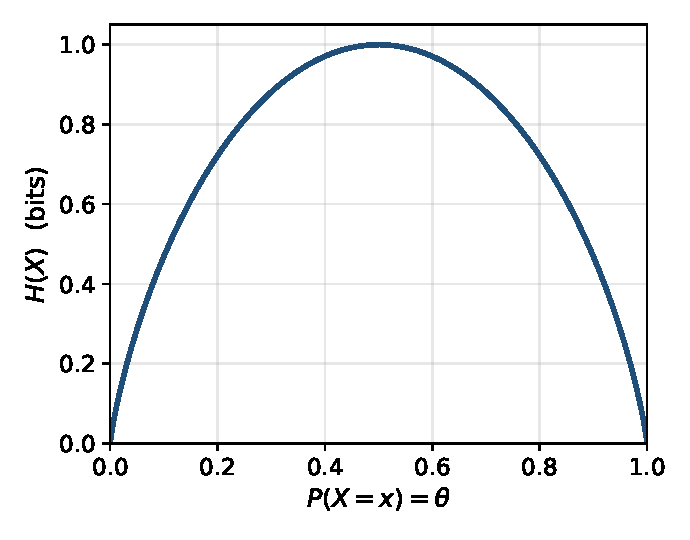
\includegraphics[width=0.5\textwidth]{entropy_coin}
\end{center}

The entropy is maximized (equal to exactly 1 bit) for a \emph{fair} coin,
$\theta = 1/2$: this is the hardest case to compress, since both outcomes are
equally likely and equally surprising. When $\theta = 0$ or $\theta = 1$, the
entropy is zero bits, because we already know the (deterministic) outcome of
a two-headed (or two-tailed) coin, so observing a flip provides no
information at all.

\framebreak

\textit{Note on units.} Here we define entropy using the binary logarithm
$\log_2$, so the result is measured in \textbf{bits}. Sometimes entropy is
instead defined using the natural logarithm $\ln$, giving the same
quantity but measured in \textbf{nats}. The two definitions agree up to a
fixed multiplicative constant ($\ln 2 \approx 0.693$).

\begin{exampleblock}{Example 2.5.3 (Entropy of horse betting)}
Suppose a gambler is listening to the results of a horse race with $N$
competitors, all equally likely to win. Since the identity of the winning
horse is the only information conveyed, and all $N$ outcomes are equally
likely, we could encode each horse with a codeword of length $\lceil \log_2
N \rceil$ bits (the ceiling $\lceil \cdot \rceil$ rounds up to the nearest
whole number of bits, since codeword lengths must be integers).
\end{exampleblock}

The complexity of the horses' \emph{names} is irrelevant here: from the
perspective of entropy, all that matters is the number of bits required to
identify which message (which horse) was received, not the intrinsic
complexity of the message's content. If instead the winning probabilities
are highly skewed (unequal), we could do better than a uniform-length code:
assign short codewords to likely outcomes and long codewords to unlikely
outcomes, giving a shorter \emph{average} codeword length than the uniform
scheme.\footnote{Samuel Morse anticipated this idea about a century before
Shannon: he counted letter frequencies in English books and gave short
codewords to common letters (E gets the single dot ``.'', I gets ``..''),
while rare letters like Q and X get longer codewords (``--.-'' and
``-..-'').}

\framebreak

\begin{block}{Remark 2.5.4 (Entropy of English)}
Shannon (1951) estimated the entropy of the English language with a
guessing game: an experimenter has a hidden message $x_1,\ldots,x_n$, and a
subject repeatedly guesses the first symbol until correct, then the second
symbol, and so on. The number of guesses $g_i$ needed for each symbol $x_i$
is recorded.
\end{block}

\textbf{Plain-English explanation.} A subject fluent in English has a strong
intuition for the statistics of the language: given the letters ``TH...'',
most people would guess ``E'' next. If the guesser's model of English is
good, the guess counts $g_i$ will mostly be small numbers, showing that
English text is highly redundant (predictable). A second subject who is only
given the sequence of guess counts $g_{1:n}$ can play the same game in
reverse and recover the original message, so the sequence of guess counts is
itself an encoding of the message.

Example sequence from the book (guessing the sentence ``THERE-IS-NO-REVERSE-ON-A-MOTORCYCLE-''):
\[
\begin{array}{l l}
x_{1:n}: & \texttt{T H E R E - I S - N O - R E V E R S E - O N - A - M O T O R C Y C L E -} \\
g_{1:n}: & 1\ 1\ 1\ 5\ 1\ 1\ 2\ 1\ 1\ 2\ 1\ 1\ 15\ 1\ 17\ 1\ 1\ 1\ 2\ 1\ 3\ 2\ 1\ 2\ 2\ 7\ 1\ 1\ 1\ 1\ 4\ 1\ 1\ 1\ 1\ 1
\end{array}
\]

Shannon estimated the entropy of English at roughly \textbf{0.6 to 1.3 bits
per character}; more modern estimates using larger corpora and algorithmic
(rather than human) predictors give a higher estimate of about
\textbf{1.58 bits per character}. Compare this to the na\"ive $\log_2 27
\approx 4.75$ bits per character needed if every letter (plus space) were
treated as equally likely and independent --- English is far more
compressible than that naive bound suggests.
\end{frame}

%% ==================================================================
\begin{frame}[fragile]{Python: Computing Shannon Entropy (1/2)}
\begin{lstlisting}[style=python]
import numpy as np

def entropy_bits(probs):
    """H(P) = sum_i p_i * log2(1/p_i), with 0*log2(1/0) := 0."""
    probs = np.asarray(probs, dtype=float)
    probs = probs[probs > 0]           # drop zero-probability outcomes
    return float(np.sum(probs * np.log2(1.0 / probs)))

# Example 2.5.2: biased coin, theta = P(Heads)
for theta in [0.5, 0.9, 0.99, 1.0]:
    H = entropy_bits([theta, 1 - theta]) if theta < 1 else 0.0
    print(f"theta={theta:5.2f}  H(X) = {H:.4f} bits")
# theta= 0.50  H(X) = 1.0000 bits   <- fair coin: maximal uncertainty
# theta= 0.90  H(X) = 0.4690 bits
# theta= 0.99  H(X) = 0.0808 bits
# theta= 1.00  H(X) = 0.0000 bits   <- deterministic: no information
\end{lstlisting}
\end{frame}

%% ==================================================================
\begin{frame}[fragile]{Python: Computing Shannon Entropy (2/2)}
\begin{lstlisting}[style=python]
# Example 2.5.3: horse race with N equally-likely competitors
for N in [2, 8, 13, 36]:
    H = entropy_bits(np.ones(N) / N)
    codeword_len = int(np.ceil(np.log2(N)))
    print(f"N={N:3d} horses: H = {H:.3f} bits, "
          f"uniform codeword length = ceil(log2 N) = {codeword_len} bits")
# N=  2 horses: H = 1.000 bits, uniform codeword length = 1 bits
# N=  8 horses: H = 3.000 bits, uniform codeword length = 3 bits
# N= 13 horses: H = 3.700 bits, uniform codeword length = 4 bits
# N= 36 horses: H = 5.170 bits, uniform codeword length = 6 bits
\end{lstlisting}

\medskip
The horse-race code length matches Example 2.5.3's uniform codeword bound
$\lceil \log_2 N \rceil$ exactly, while the entropy $H$ (which need not be
an integer) is always $\le$ that bound.
\end{frame}

%% ==================================================================
%% ================  2.5.2  SHANNON-FANO CODE  =====================
%% ==================================================================
\begin{frame}[allowframebreaks]{2.5.2 Codes and Prefix Codes}

Often we wish to encode a message over an alphabet (for instance
$\Sigma = \{\texttt{a}, \texttt{b}, \ldots, \texttt{z}\}$) into a binary
string. We define an encoding (a \emph{code}) for each character in the
alphabet, and then encode a longer string by encoding each character
separately.

Suppose we have a discrete random variable $X = (\Sigma, \bbP)$ with symbols
$\Sigma = \{x_1, \ldots, x_n\}$ and probabilities $P = \{p_1, \ldots, p_n\}$
such that $\bbP(X{=}x_i) = p_i$. Without loss of generality, all $p_i > 0$
(we discard zero-probability symbols, since they never need a codeword), and
the symbols are indexed in decreasing order of likelihood,
$p_1 \geq p_2 \geq \ldots \geq p_n$. For $i = 1,\ldots,n$, let
$F_i = \sum_{k=1}^{i-1} p_k$ be the cumulative probability up to symbol
$i-1$, so that $0 = F_1 < F_2 < \ldots < F_n = 1 - p_n$.

\framebreak

\begin{block}{Definition 2.5.6 (Code)}
Given a set of source words $S$, a \textbf{code} $C : S \to \mathbb{B}^*$ is
a function mapping messages to binary strings. The set of all encoded
messages $C(S)$ is called a set of \textbf{codewords}. A code is
\textbf{uniquely decodable} if $C$ is injective (one-to-one), and
\textbf{prefix} (or prefix-free) if $C(M)$ is a prefix-free set --- meaning
no codeword is a prefix (an initial segment) of another codeword.
\end{block}

\textbf{Plain-English explanation.} Here $\mathbb{B}^* = \{0,1\}^*$ denotes
the set of all finite binary strings (sequences of 0s and 1s of any length).
``Uniquely decodable'' just means two different messages can never produce
the identical encoded string. ``Prefix-free'' is a stronger and very useful
property: it guarantees that as soon as the decoder sees a complete
codeword go by, it can be certain that codeword has ended --- no codeword
can be the beginning of a longer codeword, so there is never any ambiguity
about where one codeword stops and the next starts.

We usually want prefix codes, because they remain uniquely decodable even
when several codewords are concatenated together, and decoding can be done
in a single left-to-right pass using at most constant memory overhead (no
need to look ahead).

\framebreak

\begin{block}{Definition 2.5.7 (Shannon-Fano code)}
Given $\Sigma$ and $P$ as above, the \textbf{Shannon-Fano} code $C : \Sigma
\to \mathbb{B}^*$ is defined as:
\begin{enumerate}
  \item Take the binary expansion $b(F_i) = 0.b_1 b_2 \ldots$ of $F_i$.
  \item Truncate the result at $l_i$ bits, where
  \[
    l_i \;\equiv\; \ell(C(x_i)) \;:=\; \left\lceil \log_2 \frac{1}{p_i} \right\rceil. \tag{2.5.8}
  \]
\end{enumerate}
The resulting string $C(x_i) := b_1 b_2 \ldots b_{l_i}$ defines the code
associated with $x_i$.
\end{block}

\textbf{Plain-English explanation.} $F_i$ is the cumulative probability mass
of all symbols more likely than $x_i$; writing it in binary and keeping only
the first $l_i$ bits gives us the codeword for $x_i$. $l_i$, the length of
the codeword for $x_i$, is simply the number of bits needed to write
$1/p_i$, rounded up to the nearest whole bit ($\lceil\cdot\rceil$ is the
ceiling/round-up function). The symbols that are most (respectively least)
likely are assigned the shortest (respectively longest) codewords -- exactly
matching the intuition from the horse-racing example.

\framebreak

\begin{block}{Theorem 2.5.9 (The Shannon-Fano code is a prefix code)}
\end{block}

\textit{Proof.} From (2.5.8) we obtain
\[
  \log_2 \frac{1}{p_i} \;\leq\; l_i \;<\; 1 + \log_2\frac{1}{p_i}
  \qquad\text{hence}\qquad
  2^{-l_i} \;\leq\; p_i \;<\; 2^{-l_i+1}.
\]
Let $x_i, x_j$ be two different symbols with $j > i$. Then
\[
  F_j = \sum_{k=1}^{j-1}p_k = \sum_{k=i}^{j-1}p_k + \sum_{k=1}^{i-1}p_k
  \;\geq\; (j-i)p_i + F_i \;\geq\; p_i + F_i \;\geq\; 2^{-l_i} + F_i,
\]
and hence $F_j - F_i \geq 2^{-l_i}$. This implies the codewords $C(x_j)$ and
$C(x_i)$ must have a mismatched bit somewhere within the first $l_i$
positions -- if they did not, all bits $b_1 \ldots b_{l_i}$ would match,
implying $|F_j - F_i| < 2^{-l_i}$, a contradiction. Since it is impossible
for $C(x_i)$ to agree with $C(x_j)$ over the first $l_i$ bits when $j>i$,
$C(x_i)$ cannot be a prefix of $C(x_j)$. The case $j<i$ is analogous.
$\blacksquare$

\textbf{Plain-English explanation.} This proof shows algebraically that no
shorter Shannon-Fano codeword can ever be an exact prefix of a longer one:
their binary expansions are guaranteed to diverge (differ) within the length
of the shorter codeword, because their cumulative probabilities $F_i$ are
always far enough apart.

\framebreak

\begin{block}{Theorem 2.5.10 (Shannon Coding)}
The expected Shannon-Fano code length (in bits per symbol) is bounded as
\[
  H(X) \;\leq\; \bbE[\ell(C(X))] \;\equiv\; \sum_i p_i l_i \;\leq\; H(X) + 1,
\]
with $H(X)$ being the entropy per symbol of the source.
\end{block}

\textbf{Plain-English explanation.} $\bbE[\ell(C(X))] = \sum_i p_i l_i$ is
the \emph{average} number of bits used per symbol, once we weigh each
codeword length $l_i$ by how often that symbol actually occurs ($p_i$). This
theorem says the Shannon-Fano code is always within one bit of the entropy
bound $H(X)$ --- it is nearly, but not quite, optimal.

\textit{Proof.} Using (2.5.8),
\[
  H(X) = \sum_i p_i \log_2\frac{1}{p_i} \;\leq\; \sum_i p_i l_i \;<\; \sum_i p_i\Big(1+\log_2\frac{1}{p_i}\Big) \;=\; 1 + \sum_i p_i \log_2\frac{1}{p_i} \;=\; H(X)+1. \qquad\blacksquare
\]

\framebreak

\begin{exampleblock}{Example 2.5.11 (Shannon-Fano code)}
Given source words $\{1,2,3,4\}$ with respective probabilities
$\{\tfrac{6}{12}, \tfrac{3}{12}, \tfrac{2}{12}, \tfrac{1}{12}\}$, we compute
the Shannon-Fano code as shown:
\end{exampleblock}

\begin{center}
\begin{tabular}{|c|c|c|c|c|c|}
\hline
$n$ & $p_n$ & $F_n$ & $b(F_n)$ & $\log_2[1/p_n]$ & $\ell(C(n))$ \quad $C(n)$ \\
\hline
1 & $6/12$  & $0$     & $.0$        & $1$              & 1 \quad 0 \\
2 & $3/12$  & $6/12$  & $.1$        & $2$              & 2 \quad 10 \\
3 & $2/12$  & $9/12$  & $.11$       & $\log_2 6 \doteq 2.6$   & 3 \quad 110 \\
4 & $1/12$  & $11/12$ & $.11101$    & $\log_2 12 \doteq 3.6$  & 4 \quad 1110 \\
\hline
\end{tabular}
\end{center}

Here the underlined digit in $.11\underline{1}01$ marks where the binary
expansion of $F_4 = 11/12$ is truncated to $l_4 = 4$ bits. We will often use
phrases such as ``$x$ has code length $-\log P(x)$'' to mean that there
exists a code $C(x)$, e.g.\ a Shannon-Fano code with respect to $P$, such
that $\ell(C(x)) = \lceil -\log P(x) \rceil$.
\end{frame}

%% ==================================================================
\begin{frame}[fragile]{Python: Building a Shannon-Fano Code (1/2)}
\begin{lstlisting}[style=python]
import math

def shannon_fano(probs):
    """Construct the Shannon-Fano code for a list of probabilities.
    Returns a list of (p_i, F_i, length_i, codeword_i)."""
    # 1. sort symbols by decreasing probability (as required by the theorem)
    order = sorted(range(len(probs)), key=lambda i: -probs[i])
    p = [probs[i] for i in order]
    rows = []
    F = 0.0
    for pi in p:
        l_i = math.ceil(math.log2(1 / pi))                 # eq. (2.5.8)
        # binary expansion of F, truncated to l_i bits
        bits, x = [], F
        for _ in range(l_i):
            x *= 2
            bit = 1 if x >= 1 else 0
            bits.append(bit)
            x -= bit
        codeword = ''.join(map(str, bits))
        rows.append((pi, F, l_i, codeword))
        F += pi
    return rows
\end{lstlisting}
\end{frame}

%% ==================================================================
\begin{frame}[fragile]{Python: Building a Shannon-Fano Code (2/2)}
\begin{lstlisting}[style=python]
# Example 2.5.11
probs = [6/12, 3/12, 2/12, 1/12]
for pi, Fi, li, cw in shannon_fano(probs):
    print(f"p={pi:.4f}  F={Fi:.4f}  l={li}  codeword={cw}")
# p=0.5000  F=0.0000  l=1  codeword=0
# p=0.2500  F=0.5000  l=2  codeword=10
# p=0.1667  F=0.7500  l=3  codeword=110
# p=0.0833  F=0.9167  l=4  codeword=1110

avg_len = sum(pi * li for pi, _, li, _ in shannon_fano(probs))
H = -sum(pi * math.log2(pi) for pi in probs)
print(f"H(X) = {H:.4f} bits,  E[length] = {avg_len:.4f} bits")
# H(X) = 1.7500 bits,  E[length] = 1.8333 bits  (within 1 bit of H(X), as guaranteed)
\end{lstlisting}
\end{frame}

%% ==================================================================
%% ==========  2.5.3  KULLBACK-LEIBLER DIVERGENCE  =================
%% ==================================================================
\begin{frame}[allowframebreaks]{2.5.3 The Kullback--Leibler Divergence}

A quantity closely related to Shannon entropy is the Kullback--Leibler (KL)
divergence, which is a measure of the ``distance'' between two probability
measures.

\begin{block}{Definition 2.5.12 (KL divergence)}
The Kullback--Leibler divergence $\mathrm{KL}$ between discrete probability
measure $P$ and semi-probability $Q$, both over $\mathcal{X}$, is defined as
\[
  \mathrm{KL}(P\|Q) \;:=\; \sum_{x \in \mathcal{X}} P(x) \log_2 \frac{P(x)}{Q(x)},
\]
where $p \log_2 \tfrac{p}{0} = \infty$ for $p > 0$, but $0 \log_2 \tfrac{0}{q} := 0$ for $q > 0$.
\end{block}

\textbf{Plain-English explanation.} A ``semi-probability'' $Q$ is like a
probability distribution except its total mass $\sum_x Q(x)$ is allowed to
be $\le 1$ rather than exactly $1$. $\mathrm{KL}(P\|Q)$ measures how much
$Q$ differs from the ``true'' distribution $P$: it is a weighted average
(weighted by $P$) of the log-ratio $\log_2\!\big(P(x)/Q(x)\big)$, which is
large and positive whenever $Q$ badly underestimates the true probability
of an outcome $x$. Like the entropy in Definition 2.5.1, we measure KL
divergence in bits here (using $\log_2$); a natural-log ($\ln$) version is
used later in the book because it is more convenient algebraically.

\framebreak

\textbf{Motivation of the KL divergence.} It may not be obvious why this
expression is a suitable ``distance''. Consider a discrete random variable
$X$ with true probability $P$. The length of the near-optimal Shannon-Fano
code (Theorem 2.5.10) for $x \in \mathcal{X}$ with respect to $P$ is, within
one bit, $h_P(x) := -\log_2 P(x)$. Now suppose $P$ is unknown, and $Q$ is
our best guess of the true probabilities. The Shannon-Fano code
(Definition 2.5.7) for $X$ using the (wrong) distribution $Q$ has length,
within one bit, $h_Q(x) := -\log_2 Q(x)$.

Coding with respect to the wrong distribution incurs a penalty (regret) of
requiring $h_Q(x) - h_P(x)$ more bits than optimal coding. The
\emph{expected regret}, called \emph{redundancy}, is
\[
  \bbE_P[h_Q(x) - h_P(x)] \;=\; \sum_{x \in \mathcal{X}} P(x)\big[\log_2 P(x) - \log_2 Q(x)\big] \;\equiv\; \mathrm{KL}(P\|Q).
\]

\textbf{Plain-English explanation.} $\bbE_P[\cdot]$ denotes an average taken
with respect to the true distribution $P$. This equation shows that
$\mathrm{KL}(P\|Q)$ is exactly the average number of \emph{extra} bits per
symbol that we waste, on average, if we design our Shannon-Fano (or Huffman)
code using the wrong distribution $Q$ instead of the true distribution $P$.
As we will see shortly, this quantity is always non-negative (Corollary
2.5.16), so coding with respect to the wrong distribution can only increase
(on average) the code length -- never decrease it.

\framebreak

\begin{exampleblock}{Example 2.5.13 (KL divergence between a biased and a fair coin)}
Consider biased coins with bias $p$ and $q$ respectively. Writing $P =
(p, 1-p)$ and $Q = (q, 1-q)$ for their distributions,
\[
  \mathrm{KL}(P\|Q) \;=\; p\log_2\frac{p}{q} + (1-p)\log_2\frac{1-p}{1-q}.
\]
\end{exampleblock}

\begin{center}
  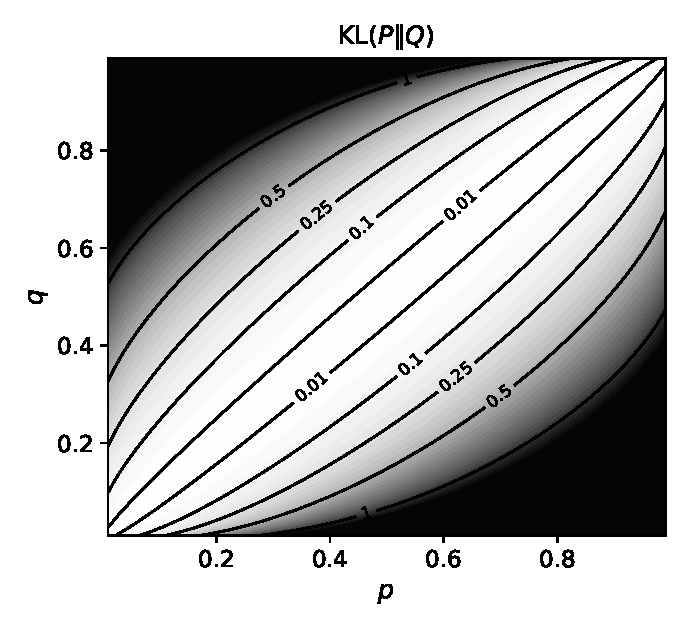
\includegraphics[width=0.42\textwidth]{kl_contour}
  \hspace{0.5cm}
  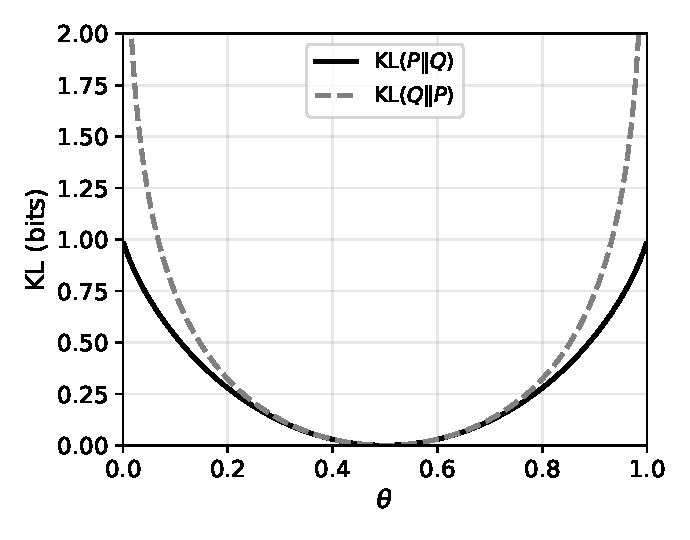
\includegraphics[width=0.42\textwidth]{kl_cross_section}
\end{center}

\textbf{Left:} $\mathrm{KL}(P\|Q)$ as a function of both biases $p$ and $q$
(contour plot; darker = larger). \textbf{Right:} a cross-section with one
coin's bias fixed at $0.5$ (a fair coin) and the other bias $\theta$
(pronounced ``theta'') varying along the horizontal axis, comparing
$\mathrm{KL}(P\|Q)$ (solid) against $\mathrm{KL}(Q\|P)$ (dashed, with roles
of $P,Q$ swapped).

\framebreak

Plotting reveals that KL is \emph{not} a symmetric function: mirroring the
contour plot over the line $p=q$ produces a visibly different picture.
Looking at the cross-section, while $\mathrm{KL}(P\|Q)$ and
$\mathrm{KL}(Q\|P)$ are similar in the neighbourhood of $\theta = 1/2$,
symmetry clearly breaks down as $\theta \to 0$ or $\theta \to 1$. In the
cross-section shown, $\mathrm{KL}(P\|Q)$ (solid, fixed reference $Q$) stays
finite and bounded, while $\mathrm{KL}(Q\|P)$ (dashed, fixed reference $P$)
diverges to infinity as $\theta \to 0$ or $\theta \to 1$.

\textbf{Asymmetry of the KL divergence.} Suppose $P$ is the true
distribution, and we are fitting an approximation $Q$ to $P$ by minimizing a
KL divergence. Since KL is not symmetric, there are two different choices,
called the \emph{forward divergence} $\mathrm{KL}(P\|Q)$ and the
\emph{reverse divergence} $\mathrm{KL}(Q\|P)$:

\begin{itemize}
  \item \textbf{Forward, $\mathrm{KL}(P\|Q) = \sum_x P(x)\log\tfrac{P(x)}{Q(x)}$:}
    $Q$ only appears in the denominator. At points $x$ where $P(x)=0$ (never
    sampled from the truth), the choice of $Q(x)$ is irrelevant. But if
    $P(x) > 0$ and $Q(x) = 0$, the ratio diverges to $\infty$. So minimizing
    $\mathrm{KL}(P\|Q)$ forces $Q$ to ``cover'' the \emph{entire} support of
    $P$ -- it must place some probability mass everywhere $P$ does.
  \item \textbf{Reverse, $\mathrm{KL}(Q\|P) = \sum_x Q(x)\log\tfrac{Q(x)}{P(x)}$:}
    any point where $Q(x)=0$ contributes nothing. But since $Q$ is a
    probability distribution, its mass must go \emph{somewhere}; if
    $P(x)=0$ there, $Q$ is forced to zero there too (to avoid the ratio
    diverging). This means minimizing $\mathrm{KL}(Q\|P)$ makes $Q$ avoid
    stretching over regions where $P(x)\approx 0$ -- it tends to
    ``mode-seek'', locking onto a single region of high probability under
    $P$ rather than spreading across all of them.
\end{itemize}

\framebreak

\begin{exampleblock}{Example 2.5.14 ($\mathrm{KL}(P\|Q)$ vs.\ $\mathrm{KL}(Q\|P)$)}
Consider a mixture of two two-dimensional Gaussians $P$, and restrict $Q =
\mathcal{N}(\boldsymbol{\mu}, \boldsymbol{\Sigma})$ to a single
two-dimensional Gaussian. Since $x \in \bbR^2$ is continuous, we replace the
sum in the KL definition by an integral. The minimizing parameters
$\boldsymbol{\mu} \in \bbR^2$ (pronounced ``mu'', the mean vector) and
$\boldsymbol{\Sigma} \in \bbR^{2\times 2}$ (pronounced ``sigma'', the
covariance matrix) can be found numerically.
\end{exampleblock}

\begin{center}
  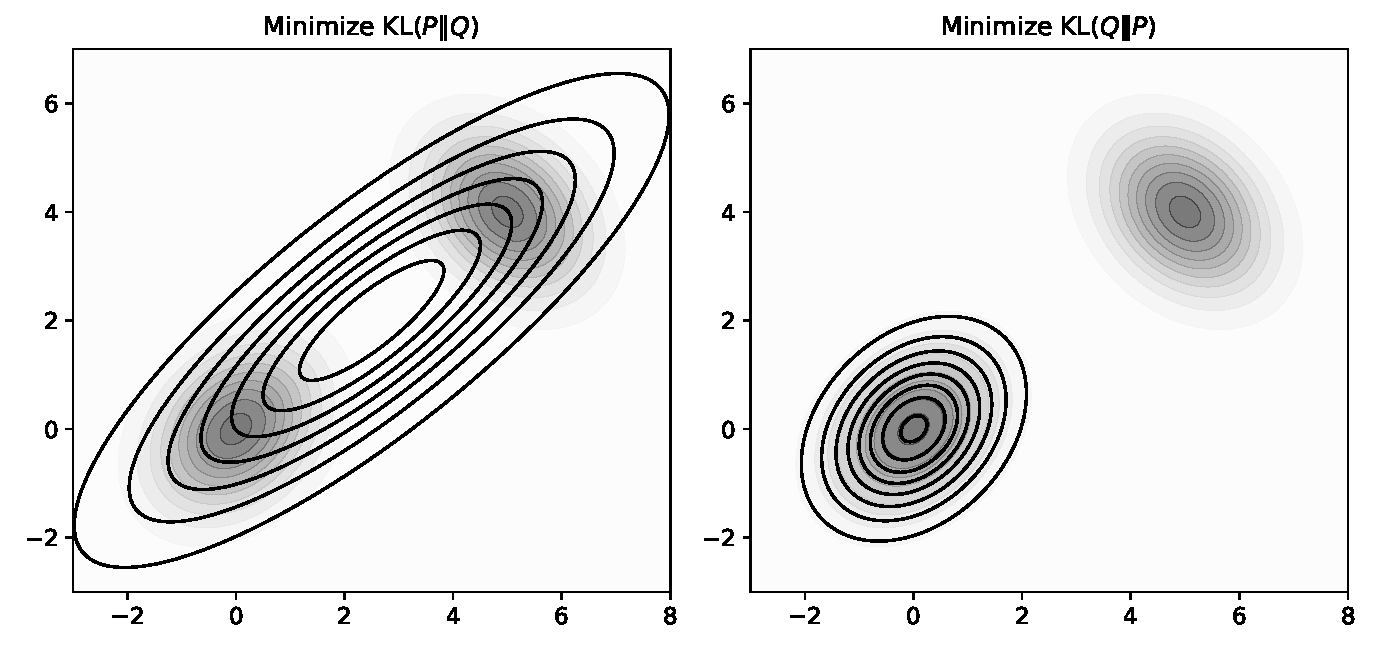
\includegraphics[width=0.85\textwidth]{gaussian_kl_asymmetry}
\end{center}

Looking at the result: $\arg\min_Q \mathrm{KL}(P\|Q)$ (left) tends to
\textbf{stretch} to cover the full support of $P$ (the shaded two-lobed
mixture), producing one broad, elongated Gaussian straddling both lobes.
Whereas $\arg\min_Q \mathrm{KL}(Q\|P)$ (right) \textbf{focuses on one of the
two lobes}, entirely ignoring the other and avoiding the low-density region
in between -- exactly the mode-seeking / mode-covering distinction described
above.

\framebreak

Without any constraint on $Q$, both KL divergences are minimized by $Q=P$,
and in that trivial case the choice of forward vs.\ reverse does not matter.
But under \emph{model misspecification} (when $Q$ is restricted to some
smaller family that cannot represent $P$ exactly, briefly discussed in
Section 3.4 of the book), the minimizing $Q$ will generally differ between
the two divergences, as the example above shows.

Noticeably, the KL divergence is \textbf{not a metric}: it is neither
symmetric, nor does it satisfy the triangle inequality. It does, however,
satisfy the property that $\mathrm{KL}(P\|Q) = 0$ if and only if $P=Q$,
which is why we still call it a ``divergence''. This does not stop it from
being invaluable in the chapters to come. We also note that KL is always
\textbf{non-negative}, as a corollary of the following theorem.

\framebreak

\begin{block}{Theorem 2.5.15 (Gibbs inequality)}
Given discrete probability $\{p_1,\ldots,p_N\}$ ($\sum_i p_i = 1$) and
semi-probability $\{q_1,\ldots,q_N\}$ ($\sum_i q_i \leq 1$), we have
\[
  \sum_{i=1}^{N} p_i \log_2 p_i \;\geq\; \sum_{i=1}^{N} p_i \log_2 q_i,
\]
defining $p\log_2 0 = -\infty$ for $p>0$ but $0\log_2 0 := 0$ as before.
Equality holds iff $p_i = q_i$ for all $i$.
\end{block}

\textit{Proof.} If any $q_i=0$ (with $p_i > 0$) the bound trivially holds
(right side is $-\infty$), so suppose all $q_i > 0$. Then, discarding terms
with $p_i = 0$,
\[
  \sum_i p_i \ln\frac{q_i}{p_i} \;\leq\; \sum_i p_i\Big(\frac{q_i}{p_i}-1\Big) \;=\; \sum_i [q_i - p_i] \;\leq\; 1-1 \;=\; 0,
\]
using $\ln x \leq x-1$ for all $x>0$. Dividing by $\ln 2$ gives $\sum_i p_i
\log_2[q_i/p_i] \leq 0$, which rearranges to Gibbs' inequality. Equality in
$\ln x \le x - 1$ holds only at $x=1$, i.e.\ we need $q_i/p_i = 1$, i.e.\
$p_i = q_i$. $\blacksquare$

\begin{block}{Corollary 2.5.16 (KL divergence is non-negative)}
The KL divergence $\mathrm{KL}(P\|Q)$ is non-negative, and is zero iff
$P=Q$.
\end{block}

\textit{Proof.} Both properties follow immediately by applying Gibbs'
inequality with $p_i = P(x_i)$ and $q_i = Q(x_i)$. $\blacksquare$
\end{frame}

%% ==================================================================
\begin{frame}[fragile]{Python: KL Divergence and Its Asymmetry (1/2)}
\begin{lstlisting}[style=python]
import numpy as np

def kl_divergence(P, Q):
    """KL(P||Q) in bits, for discrete distributions given as arrays."""
    P, Q = np.asarray(P, dtype=float), np.asarray(Q, dtype=float)
    mask = P > 0                                   # 0*log2(0/q) := 0
    return float(np.sum(P[mask] * np.log2(P[mask] / Q[mask])))

# Example 2.5.13: biased vs fair coin, p = 0.9, q = 0.5
p, q = 0.9, 0.5
P, Q = [p, 1 - p], [q, 1 - q]
print("KL(P||Q) =", kl_divergence(P, Q))   # regret of using Q when truth is P
print("KL(Q||P) =", kl_divergence(Q, P))   # regret of using P when truth is Q
# KL(P||Q) = 0.5310 bits
# KL(Q||P) = 0.6098 bits   <- confirms KL is NOT symmetric

# Verify Gibbs' inequality / non-negativity (Corollary 2.5.16) numerically
rng = np.random.default_rng(0)
for _ in range(5):
    P = rng.dirichlet(np.ones(4))          # random probability vector
    Q = rng.dirichlet(np.ones(4))
    kl = kl_divergence(P, Q)
    print(f"KL(P||Q) = {kl:.4f}  (always >= 0: {kl >= -1e-12})")
# every printed KL value is >= 0, confirming Corollary 2.5.16 empirically
\end{lstlisting}
\end{frame}

%% ==================================================================
\begin{frame}[fragile]{Python: KL Divergence and Its Asymmetry (2/2)}
\begin{lstlisting}[style=python]
# Redundancy interpretation: KL(P||Q) = E_P[ -log2 Q(x) - (-log2 P(x)) ]
P = np.array([0.9, 0.1])
Q = np.array([0.5, 0.5])
h_Q = -np.log2(Q)                          # code length under WRONG dist. Q
h_P = -np.log2(P)                          # code length under TRUE dist. P
redundancy = np.sum(P * (h_Q - h_P))
print("redundancy =", redundancy, " == KL(P||Q) =", kl_divergence(P, Q))
# redundancy = 0.5310  == KL(P||Q) = 0.5310   <- matches, as proved above
\end{lstlisting}

\medskip
This confirms the motivation derivation from earlier: the extra bits wasted
by coding with the wrong distribution $Q$ instead of the truth $P$ (the
\emph{redundancy}) is exactly $\mathrm{KL}(P\|Q)$, computed here two
different ways with matching results.
\end{frame}

%% ==================================================================
%% ==============  2.5.4  THE KRAFT INEQUALITY  ====================
%% ==================================================================
\begin{frame}[allowframebreaks]{2.5.4 The Kraft Inequality}

Earlier we discussed prefix codes and gave some motivation as to why we
might want to use them. One important property of prefix codes is the Kraft
inequality.

\begin{block}{Theorem 2.5.17 (Kraft inequality)}
Let $b_1, b_2, \ldots$ be a finite or infinite sequence of binary strings.
There exists a prefix code $\mathcal{C} = \{c_1, c_2, \ldots\}$ such that
$\ell(b_n) = \ell(c_n)$ for all $n$ if and only if
\[
  \sum_n 2^{-\ell(b_n)} \;\leq\; 1.
\]
\end{block}

\textbf{Plain-English explanation.} $\ell(b_n)$ denotes the length (number
of bits) of the string $b_n$. The theorem says: a list of desired codeword
\emph{lengths} $\ell(b_1), \ell(b_2), \ldots$ can be realized by \emph{some}
valid prefix code if and only if the sum of $2^{-\ell(b_n)}$ over all
codewords does not exceed 1. This gives us a simple, purely arithmetic test
for whether a set of codeword lengths is achievable by a prefix-free code,
without ever having to construct the code itself.

\framebreak

\textit{Proof (Only if).} Recall the standard one-to-one correspondence
between a finite binary string $x$ and the interval $I_x = [0.x,\, 0.x +
2^{-\ell(x)})$ on the real line. For each $c_n$, the length of $I_{c_n}$ is
$2^{-\ell(b_n)}$ since $c_n$ and $b_n$ have matching lengths. Because
$\mathcal{C}$ is a prefix code, the corresponding intervals are disjoint:
$I_{c_n} \cap I_{c_m} = \emptyset$ for $n \ne m$. Since the intervals are
disjoint subsets of $[0,1)$, the sum of their lengths is at most 1:
\[
  \sum_n 2^{-\ell(b_n)} \;=\; \sum_n \lambda\big([0.b_n, 0.b_n+2^{-\ell(b_n)})\big) \;=\; \lambda\Big(\bigcup_n [0.b_n, 0.b_n + 2^{-\ell(b_n)})\Big) \;\leq\; \lambda([0,1)) \;=\; 1,
\]
where $\lambda([a,b)) := b-a$ denotes interval length. This proves the
inequality holds for any prefix code.

\textit{Proof (If).} Suppose $b_1, b_2, \ldots$ are given such that the
inequality holds, and (w.l.o.g.) the lengths $\ell(b_n)$ are non-decreasing.
Choose disjoint, adjacent, half-open intervals $I_1, I_2, \ldots$ from the
left end of $[0,1)$, of lengths $2^{-\ell(b_1)}, 2^{-\ell(b_2)}, \ldots$ For
each $n\geq 1$, the right end of $I_n$ is $\sum_{i=1}^n 2^{-\ell(b_i)}$,
which is exactly the left end of $I_{n+1}$. Since lengths are
non-decreasing, each interval $I_n$ equals $[0.c_n, 0.c_n + 2^{-\ell(c_n)})$
for some binary string $c_n$ of length $\ell(c_n) = \ell(b_n)$. By
construction, $\{c_1, c_2, \ldots\}$ forms a prefix code. $\blacksquare$

\framebreak

\begin{block}{Remark 2.5.18 (Kraft inequality as sum over trees)}
The Kraft inequality has a pleasing geometric interpretation: any prefix
code can be represented as a binary tree, where each codeword corresponds to
a leaf node of the tree. Assign probability mass $1$ to the root node, and
then recursively for each non-leaf node, split its probability mass in half
between its two children.
\end{block}

\textbf{Plain-English explanation.} Since the total probability mass is
unchanged by each split (or only decreases if some node has only one child
instead of two), the sum of the probabilities assigned to all the leaf
nodes is bounded above by 1. A leaf node at depth $d$ (i.e., $d$ splits deep
into the tree) receives probability mass $2^{-d}$. Hence $\sum_n
2^{-\ell(c_n)} \leq 1$ for a prefix code $\mathcal{C} = \{c_1,\ldots,c_n\}$
--- exactly the Kraft inequality. If every internal node has either zero or
exactly two children (never just one -- this is called a \emph{perfect
tree}), the prefix code is \emph{complete} and the sum equals exactly 1.

\begin{center}
  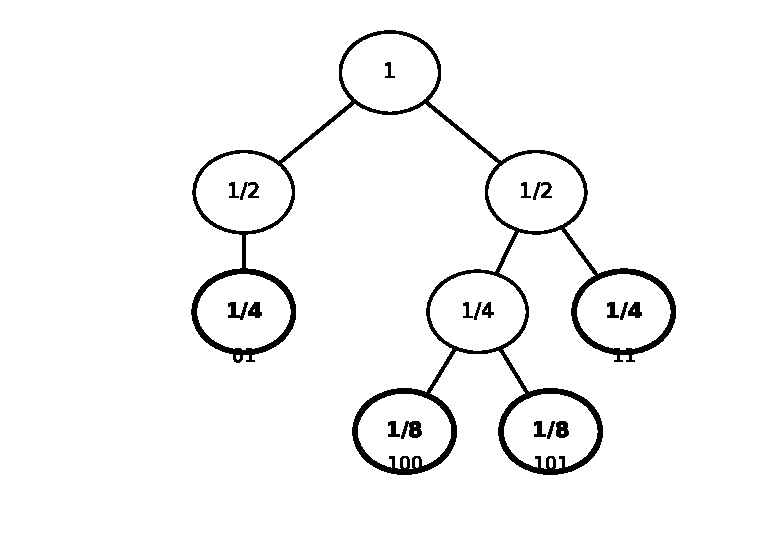
\includegraphics[width=0.55\textwidth]{kraft_tree}
\end{center}

The prefix code $\mathcal{C} = \{01, 100, 101, 11\}$ illustrated above: the
sum of the probability masses assigned to the four leaves (in bold) is
$\tfrac14+\tfrac14+\tfrac18+\tfrac18 = \tfrac34 \le 1$, confirming the Kraft
inequality (with room to spare, since this code is not yet complete --- we
could still add the codeword $00$).
\end{frame}

%% ==================================================================
\begin{frame}[fragile]{Python: Verifying the Kraft Inequality (1/2)}
\begin{lstlisting}[style=python]
def kraft_sum(lengths):
    """sum_n 2^{-length_n}; must be <= 1 for a valid prefix code to exist."""
    return sum(2.0 ** (-l) for l in lengths)

def is_prefix_free(codewords):
    """Brute-force check: no codeword is a prefix of another."""
    for i, a in enumerate(codewords):
        for j, b in enumerate(codewords):
            if i != j and b.startswith(a):
                return False
    return True

# The code from Figure 2.17 (Remark 2.5.18): C = {01, 100, 101, 11}
code = ["01", "100", "101", "11"]
lengths = [len(c) for c in code]
print("codeword lengths:", lengths)
print("prefix-free?      ", is_prefix_free(code))
print("Kraft sum = ", kraft_sum(lengths), " (<= 1 required)")
# codeword lengths: [2, 3, 3, 2]
# prefix-free?       True
# Kraft sum =  0.75  (<= 1 required)   <- satisfied, with slack 0.25
\end{lstlisting}
\end{frame}

%% ==================================================================
\begin{frame}[fragile]{Python: Verifying the Kraft Inequality (2/2)}
\begin{lstlisting}[style=python]
# Attempt an INVALID set of desired lengths: three codewords all length 1.
# Kraft's theorem says no prefix code can realize this...
bad_lengths = [1, 1, 1]
print("Kraft sum (bad) =", kraft_sum(bad_lengths), " -> exceeds 1, IMPOSSIBLE")
# Kraft sum (bad) = 1.5  -> exceeds 1, IMPOSSIBLE
# (indeed: only two length-1 binary strings exist at all, "0" and "1")
# Reconstruct a prefix code from valid lengths via the "if" direction
# of Theorem 2.5.17: place codewords left-to-right along [0,1).
def code_from_lengths(lengths):
    lengths = sorted(lengths)
    codewords, cursor = [], 0.0
    for l in lengths:
        bits, x = [], cursor
        for _ in range(l):
            x *= 2
            bit = 1 if x >= 1 else 0
            bits.append(bit)
            x -= bit
        codewords.append(''.join(map(str, bits)))
        cursor += 2.0 ** (-l)
    return codewords

print(code_from_lengths([1, 2, 3, 3]))
# ['0', '10', '110', '111']   <- a valid prefix code with these lengths
\end{lstlisting}
\end{frame}

%% ==================================================================
\begin{frame}{Summary: Section 2.5}

\begin{itemize}
  \item \textbf{Shannon information content} $h(x) = \log_2[1/P(x)]$
    measures, in bits, how surprising an outcome $x$ is; \textbf{entropy}
    $H(X) = \bbE_P[h(X)]$ is its average over the whole distribution, and
    bounds how well a source can be compressed.
  \item The \textbf{Shannon-Fano code} builds a concrete prefix code from
    cumulative probabilities, with codeword lengths $l_i = \lceil
    \log_2(1/p_i)\rceil$; its average length is always within one bit of the
    entropy: $H(X) \le \bbE[\ell(C(X))] \le H(X)+1$.
  \item The \textbf{KL divergence} $\mathrm{KL}(P\|Q) = \sum_x P(x)\log_2
    \frac{P(x)}{Q(x)}$ measures the average extra bits wasted coding with the
    wrong distribution $Q$ instead of the truth $P$; it is asymmetric,
    always non-negative (Gibbs' inequality), and zero exactly when $P=Q$.
  \item The \textbf{Kraft inequality} $\sum_n 2^{-\ell(b_n)} \le 1$ is the
    exact arithmetic condition for a set of codeword lengths to be
    realizable by some prefix-free code, with a clean interpretation as
    probability mass splitting down a binary tree.
\end{itemize}

\medskip
\textbf{Coming next in the book:} the \emph{Shannon Coding Theorem}
(Section 2.5.5) shows that an \emph{optimal} prefix code (not just
Shannon-Fano) also satisfies $H(P) \le L^*_P \le H(P)+1$; \emph{Huffman
codes} achieve this optimum exactly; and \emph{Arithmetic Coding}
(Section 2.5.6) removes the ``$+1$ bit'' penalty entirely by coding whole
sequences rather than symbol-by-symbol.
\end{frame}

\begin{frame}{References}
\begin{itemize}
  \item M.\ Hutter, D.\ Quarel, E.\ Catt. \emph{An Introduction to Universal
    Artificial Intelligence}. CRC Press, 2024. Chapter 2, Section 2.5.
  \item C.\ E.\ Shannon. ``A Mathematical Theory of Communication.'' \emph{Bell
    System Technical Journal}, 27:379--423, 1948.
  \item C.\ E.\ Shannon. ``Prediction and Entropy of Printed English.''
    \emph{Bell System Technical Journal}, 30:50--64, 1951.
  \item D.\ A.\ Huffman. ``A Method for the Construction of Minimum-Redundancy
    Codes.'' \emph{Proceedings of the IRE}, 40(9):1098--1101, 1952.
\end{itemize}
\end{frame}

\end{document}
